\chapter{Introduction}
\label{chap:introduction}
\begin{figure}[t]
    \centering
    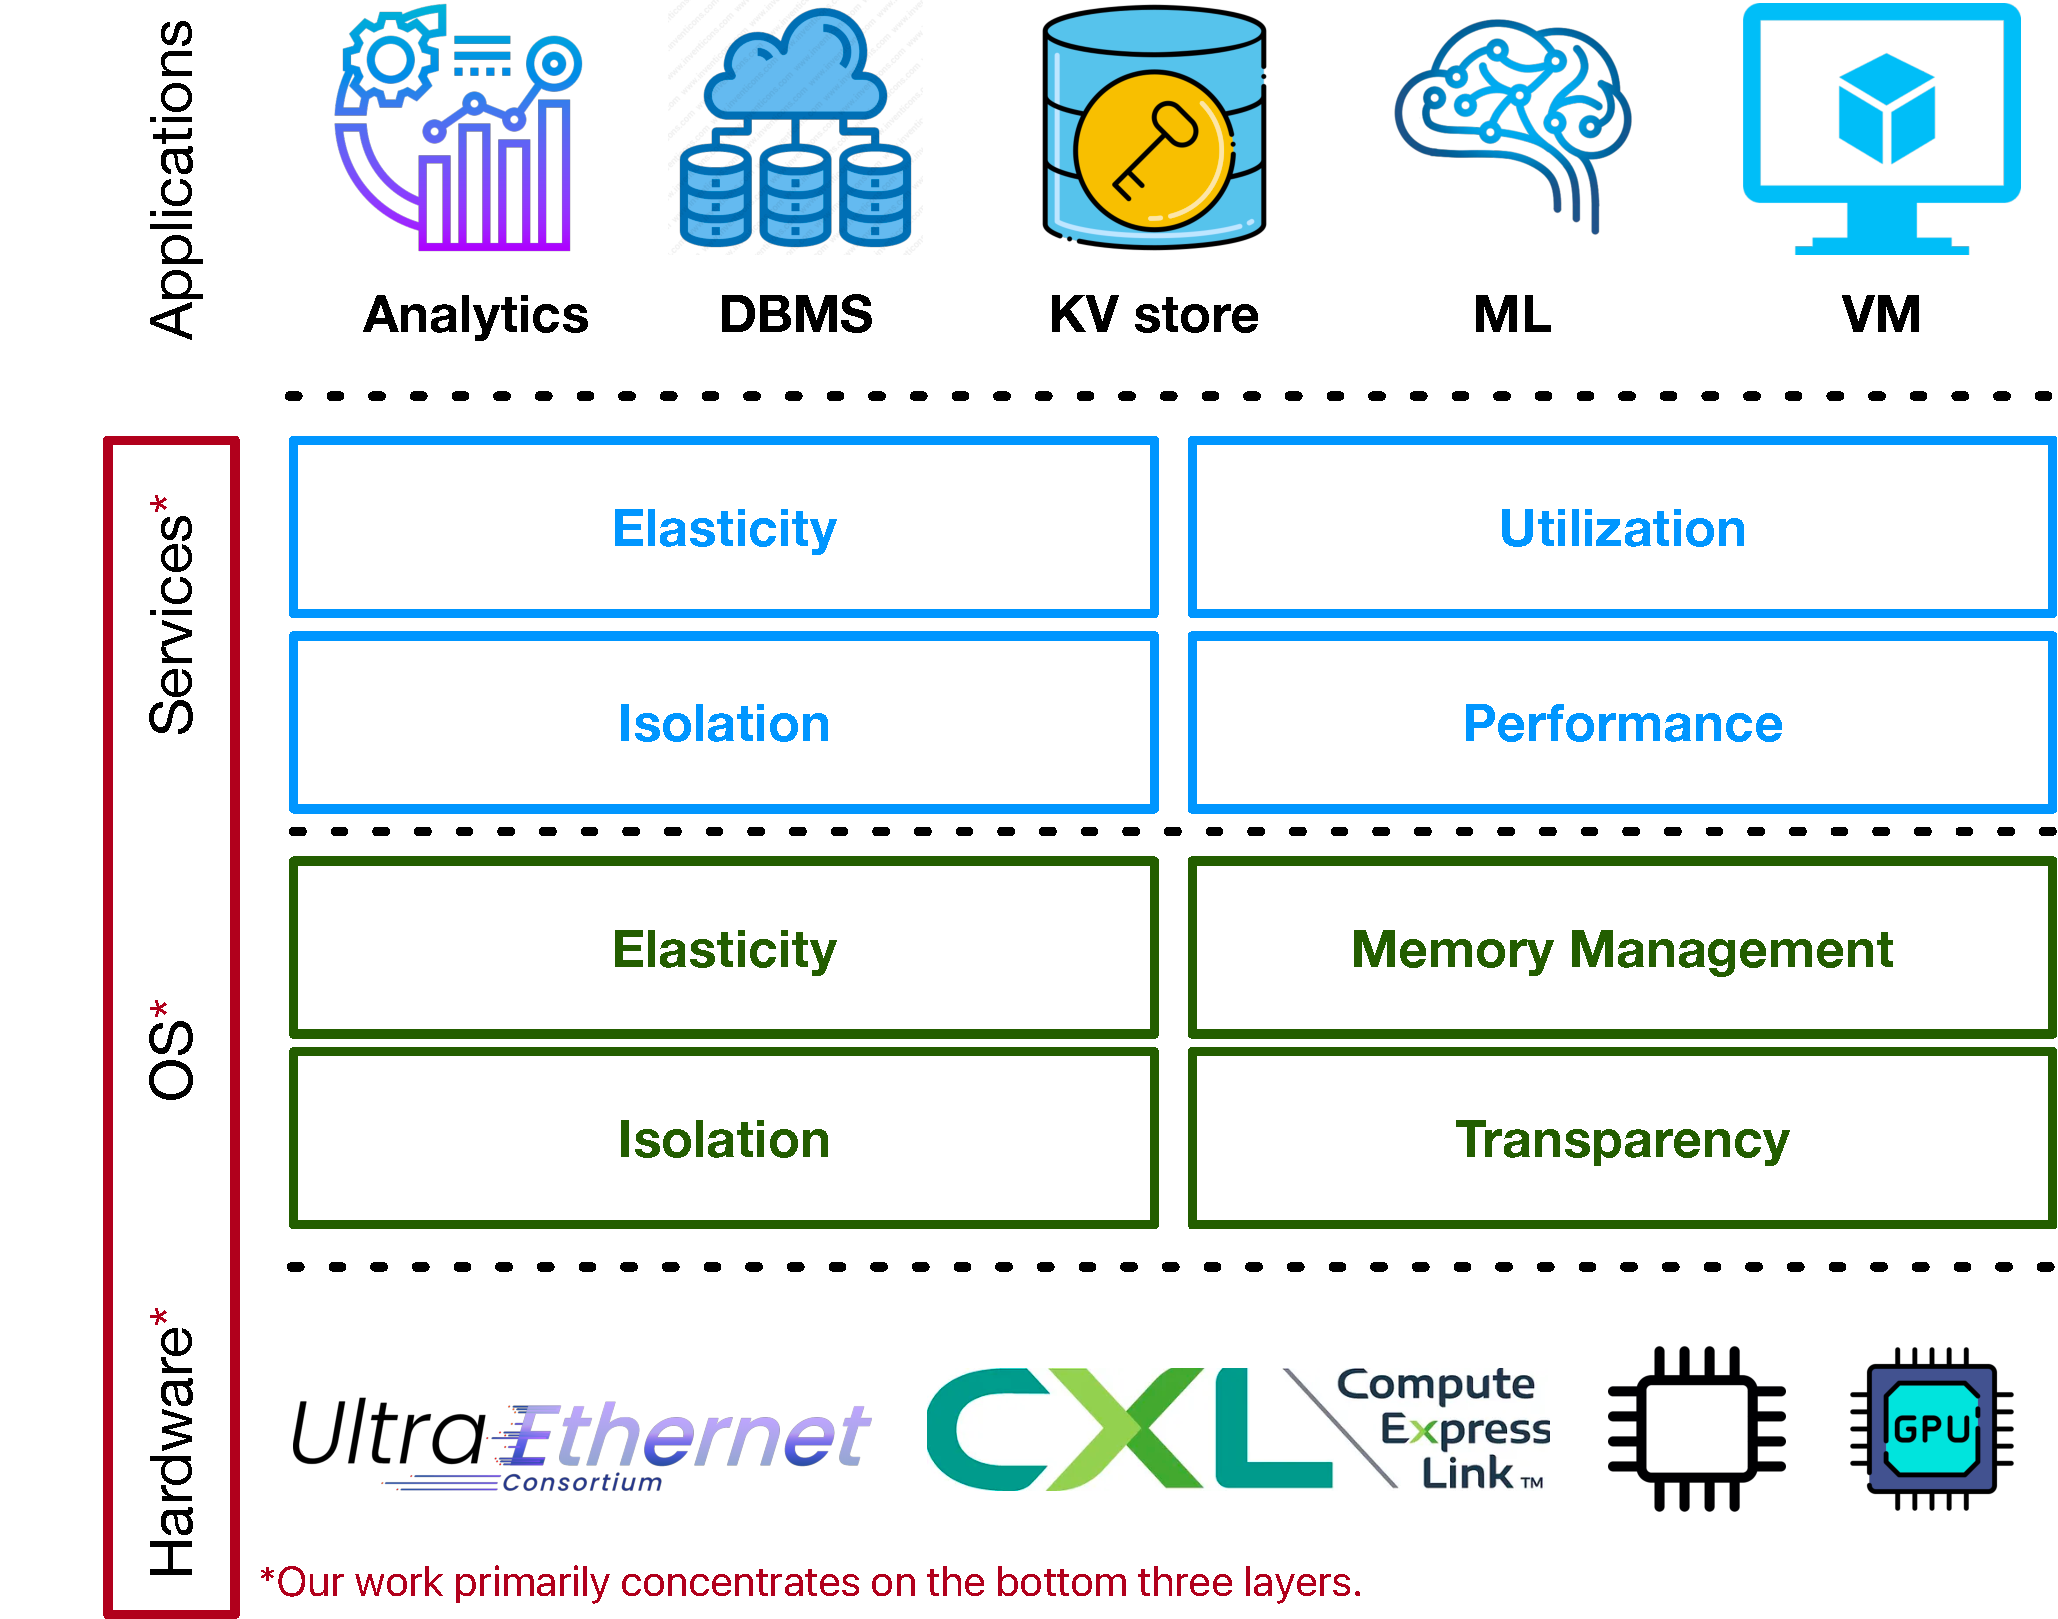
\includegraphics[width=0.8\columnwidth]{stack.pdf}
      \caption[Cloud Stack of Disaggregated Architecture]{\textbf{Cloud Stack of Disaggregated Architecture.}} \vspace{-1.0em}
      \label{fig:stack}
\end{figure}
The growing demand for scalable and efficient data center architectures has led to the emergence of resource disaggregation~\cite{mind, legoos, disagg, memdisagg1, memdisagg2, memdisagg3, memdisagg4, memdisagg5, memdisagg6}. This modern paradigm represents a significant shift from traditional monolithic server architectures. In conventional setups, servers are typically equipped with a fixed combination of compute, memory, and storage resources. In contrast, resource-disaggregated systems physically separate these resources and distribute them across various interconnects, such as networks~\cite{disagg, legoos, mind}, CXL~\cite{cxl, cxlasic}, and others. This separation allows for more flexible resource allocation and utilization.

Within the broader context of resource disaggregation in modern data center architectures, \textbf{memory disaggregation}~\cite{memdisagg1, memdisagg2, memdisagg3, memdisagg4, memdisagg5, memdisagg6} plays a crucial and foundational role. In traditional monolithic architecture, memory often becomes a bottleneck, limiting the scalability and adaptability of applications. This issue has been frequently observed and reported in production data centers~\cite{memory1, memory2, memory3, memory4, memory5, memory6, memory7, memory8, memory9, memory10}. By decoupling memory resources from compute and storage elements and presenting them as pooled, disaggregated resources~\cite{pool1, pool2}, data centers can achieve increased efficiency, scalability, and adaptability. Memory-intensive applications~\cite{redis, ramcloud, sparkmemory} can access the memory they need on demand, without being constrained by the limitations of individual servers. Memory disaggregation is the first step toward realizing the full potential of resource disaggregation, enabling data centers to efficiently allocate and utilize resources based on dynamic application needs. 


\section{Limitations of Existing Approaches}

While memory disaggregation offers numerous advantages, transitioning existing applications to this architecture is far from straightforward. Recent research has explored various approaches to tackle this challenge. Some efforts focus on optimizing applications for disaggregated memory~\cite{farm, aifm, sherman, existing1}, while others aim to transparently port applications, offloading the responsibility for mitigating performance penalties—stemming from mismatches between disaggregated architectures and traditional software interfaces—to the service or operating system layer~\cite{mind, legoos, fastswap, infiniswap, runtime1, runtime2}. Meanwhile, hardware innovations further complicate the situation. Different interconnects, such as Ethernet and CXL, offer diverse interfaces and performance characteristics, making it difficult to standardize software stack designs.


The core issue lies in the fundamental mismatch between the existing cloud stack, designed for monolithic architectures, and the requirements of disaggregated architectures (Figure \ref{fig:stack}). The current cloud and hardware stacks are not inherently aware of the unique characteristics of disaggregated memory, leading to distinct challenges across different layers of the stack:

\paragraphb{Application interface} In disaggregated architectures, applications encounter unique challenges compared to traditional monolithic systems. The key difference lies in resource distribution: compute, memory, and storage are spread across multiple resource nodes rather than centralized within a single server. This distribution necessitates complex communication and data management strategies to address increased latency and resource coordination. Transparency also becomes a critical concern. There is an inherent trade-off between the benefits of disaggregating resources and the associated performance overhead. Application developers may either significantly redesign their applications for more efficient resource utilization and management or rely on disaggregated cloud providers to integrate resource management at the service or operating system layer to ensure a smoother transition.

\paragraphb{Operating system support} Unlike monolithic servers where the operating system(OS) manages resources within a single server, the placement and function of the OS in disaggregated architectures are still subjects of debate in both industry and academia. Options include centralizing the OS at a single point~\cite{mind, chase} in the architecture or disaggregating its functions across different resource nodes~\cite{legoos}.

\paragraphb{Performance overheads} Transitioning existing applications to a disaggregated architecture transparently introduces a spectrum of performance challenges. These include, but are not limited to, managing memory partitioning~\cite{jiffy} and addressing applications with irregular memory access patterns~\cite{chase}. Various other issues, such as latency sensitivity, bandwidth limitations, and the overhead of remote resource management, compound this complexity. These factors contribute to the overall performance penalty that disaggregated systems must carefully consider and mitigate.

\paragraphb{Future interconnects} The use of networks as interconnects for resource disaggregation has been a focus of research in both academia and industry. However, networks face inherent challenges, such as performance slowdowns compared to intra-server resource access and the absence of built-in coherency. Emerging hardware technologies like Compute Express Link (CXL)~\cite{cxl, cxlasic, pond} offer promising improvements, including faster access times and hardware-supported cache coherence. Despite this potential, current hardware prototypes and software support for these technologies are still in early stages, and their full impact on software design remains uncertain.

\section{Thesis Overview}

In this dissertation, we attempt to take a top-down approach and explore the optimal memory management solutions for three most significant layers, i.e. Service, OS and Hardware layers of disaggregated memory architectures.

\subsection{Service Layer: Memory Management as a Service}
As the layer closest to the application, we first explore the design requirements and challenges of providing disaggregated memory management as a service. This service manages a pool of memory resources and exposes them to applications. We propose an end-to-end system design called Jiffy, which enables multiple applications or tasks to efficiently share memory resources in an elastic manner. Jiffy also offers interfaces for several popular data structures, making it easily applicable to existing cloud applications.

\subsection{OS Layer: In-network Near-Memory Processing}

While applications may use Jiffy to manage memory resources, we take a deeper approach by considering the Operating System (OS) as the manager of memory. This allows applications to run transparently while benefiting from the disaggregated architecture. In disaggregated systems, compute and memory resources are decoupled, meaning there is no single host, as in monolithic architectures, to handle the critical task of resource management—traditionally done by the OS. We propose a new generation OS design that embeds OS functionality within the interconnects. Starting with a system called MIND, we address fundamental challenges in memory management, such as memory address translation, memory protection, and cache coherence across multiple hosts. This resource decoupling and in-network memory management perform well for cache-friendly workloads but struggle with cache-unfriendly workloads due to the overhead of interconnect communication. To address this, we developed PULSE, a near-memory accelerator designed from the ground up. PULSE analyzes common pointer traversal applications and identifies a simple, yet effective interface that can be easily integrated into existing cloud applications.

\subsection{Hardware Layer: Memory Management for Next-Gen Interconnects}
In prior work~\cite{mind,legoos}, Ethernet has been the most commonly used interconnect for disaggregated data centers. However, with the emergence of new memory interconnects like Compute Express Link (CXL), memory management must be adapted to accommodate these new interfaces. In the context of disaggregated architectures, new challenges arise, such as how applications can effectively utilize multiple tiers of memory. To address this, we begin with a performance evaluation of CXL 1.1 extended memory in a single-host environment and explore how modern data center applications can benefit from such disaggregated memory systems.

\section{Outline and Previously Published Work}

This dissertation is organized as follows. Chapter~\ref{chap:service} introduces Jiffy, a distributed memory management system that decouples memory capacity and lifetime from compute in the serverless paradigm. Chapter~\ref{chap:os} describes two innovated system design: (1) MIND, a rack-scale memory disaggregation system that uses programmable switches to embed memory management logic in
the network fabric. (2) PULSE, a framework centered on enhancing in-network optimizations for
irregular memory accesses within disaggregated data centers. Chapter ~\ref{chap:hardware} presents our exploration in latest Compute Express Link(CXL) hardware. We conclude with our contributions and possible future work directions in Chapter~\ref{chap:future}.

Chapter~\ref{chap:service} revises material from~\cite{jiffy}\footnote{Work done in collaboration with Rachit Agarwal, Aditya Akella, and Ion Stoica}. Chapter~\ref{chap:os} revises material from~\cite{mind}\footnote{Work done in collaboration with Seung-seob Lee, Yanpeng Yu, Lin Zhong and Abhishek Bhattacharjee} and~\cite{chase}\footnote{Work done in collaboration with Seung-seob Lee and Abhishek Bhattacharjee}. Finally, Chapter~\ref{chap:hardware} revises material from~\cite{cxleurosys}\footnote{Work done in collaboration with the Bytedance Infrastructure team}.
